\chapter{Stato dell'arte}
\label{chap:statoarte}

In questo capitolo vengono introdotti alcuni progetti già esistenti che sono in qualche modo simili o correlati al progetto OpenLDAT, e in che modo differiscono da esso. Sono stati scelti a titolo esemplificativo Nvidia LDAT, DisplayCAL e il dispositivo di RTINGS usato per le loro recensioni, ma questo non è in alcun modo un elenco esaustivo. Poiché Nvidia LDAT è il progetto più simile, nel capitolo \ref{chap:outro} verrà mostrata una tabella comparativa tra Nvidia LDAT e OpenLDAT.

\section{Nvidia LDAT}
Intorno al mese di Settembre 2020, Nvidia ha distribuito un prototipo di un dispositivo chiamato Nvidia LDAT, abbreviazione di \textit{Latency Display Analysis Tool}. Questo dispositivo, che non è stato poi commercializzato, è stato una delle maggiori ispirazioni per il progetto OpenLDAT.

Il dispositivo Nvidia LDAT si presenta come una piccola scatola di plastica stampata in 3D su cui sono presenti un LED RGB che indica lo stato del dispositivo e i click, un sensore di luminosità, una porta Micro-USB per collegarlo ad un PC che esegue il software di LDAT, un connettore per un mouse modificato, una corda per poterlo appendere più facilmente al display, e un jack audio che può essere opzionalmente collegato dalla macchina di test al dispositivo. La figura \ref{fig:nvldat_front} mostra la parte frontale del dispositivo.

\begin{figure}[h!]
	\centering
	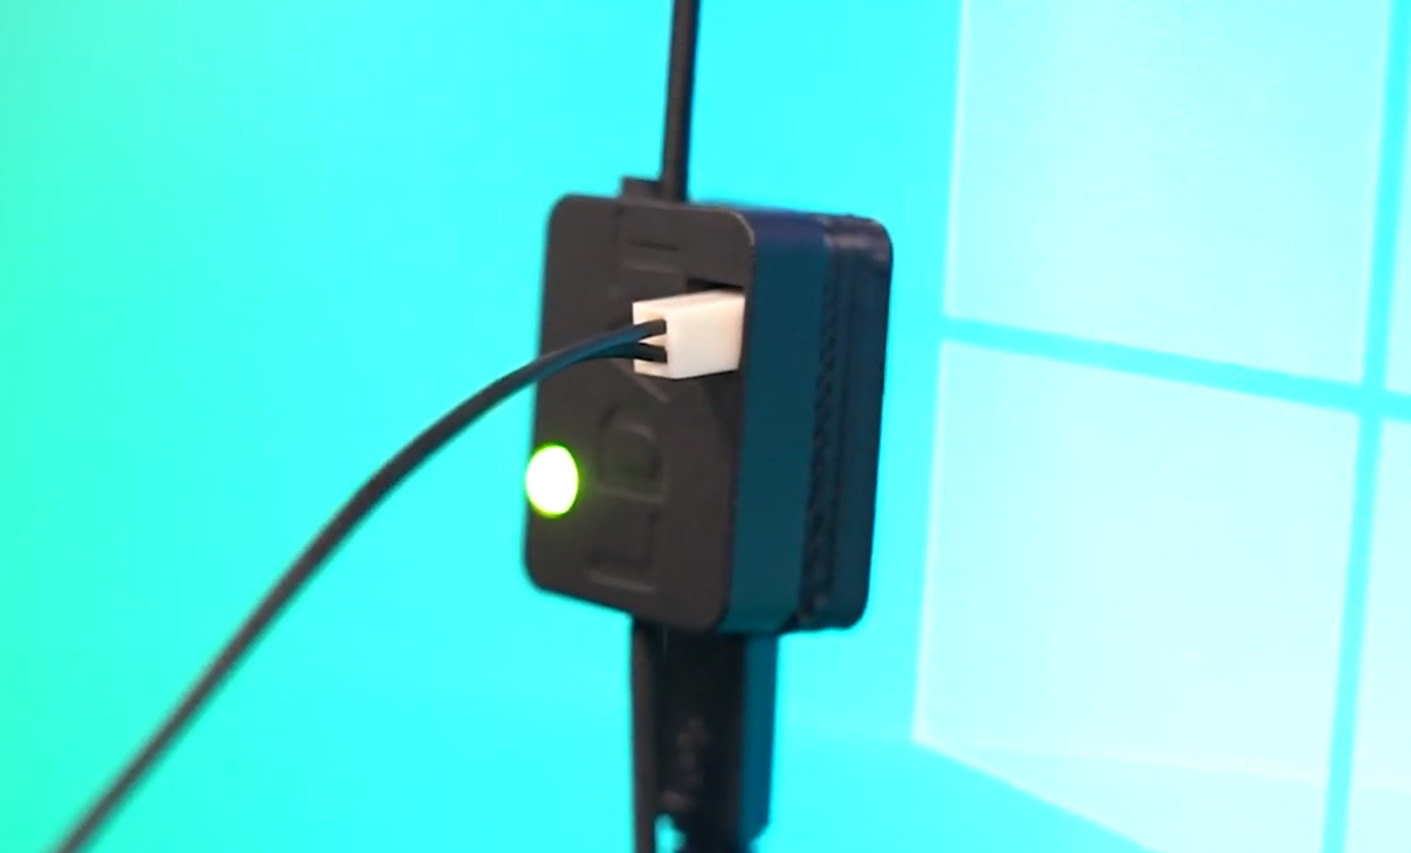
\includegraphics[width=0.8\textwidth]{StatoDellArte_files/nvldat_front.jpg}
	\caption{Parte frontale del dispositivo Nvidia LDAT (da GamersNexus)}
	\label{fig:nvldat_front}
\end{figure}

Non è noto nulla riguardo all'hardware presente all'interno, ma dall'immagine in figura \ref{fig:nvldat_back}, il sensore di luminosità sembra essere un fotodiodo piuttosto grande, o forse addirittura un CCD. Non sono stati eseguiti dei \textit{teardown} del dispositivo, probabilmente su esplicita richiesta di Nvidia, per cui non è stato possibile osservare il tipo di microcontroller o l'elettronica all'interno.

\begin{figure}[h!]
	\centering
	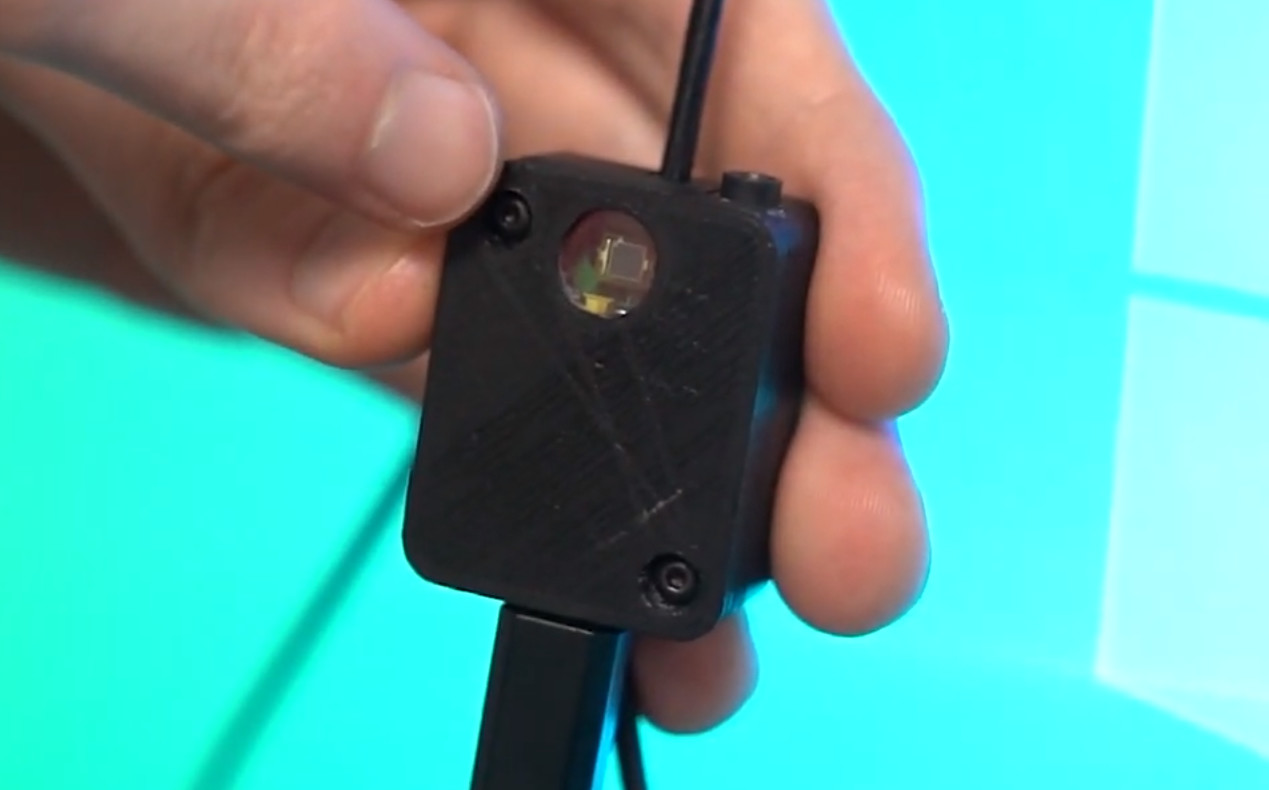
\includegraphics[width=0.8\textwidth]{StatoDellArte_files/nvldat_back.jpg}
	\caption{Parte posteriore del dispositivo Nvidia LDAT (da GamersNexus)}
	\label{fig:nvldat_back}
\end{figure}

Il software di Nvidia LDAT implementa un test per misurare quella che Nvidia chiama \textit{click-to-photon response}, ossia il tempo che passa tra la pressione di un click del mouse e il cambio di luminosità sullo schermo. Il test può essere eseguito in modo automatico, con il dispositivo che esegue i click su un'applicazione, oppure in modo manuale, utilizzando un mouse modificato collegato ai due pin sulla parte frontale del dispositivo.\\
Il software fornisce inoltre la possibilità di misurare il ritardo utilizzando l'audio catturato tramite il jack presente sul dispositivo. Questa scelta è piuttosto bizzarra, poiché la scheda audio ha una latenza diversa rispetto allo stack grafico e il display, ma può comunque fornire una stima del ritardo poiché le applicazioni processano gli input a intervalli regolari che dipendono dal framerate, per cui un'applicazione a 30 FPS avrà più ritardo di una a 60 FPS, anche sull'audio.\\
La figura \ref{fig:nvldat_software} mostra uno screenshot del software Nvidia LDAT in azione.

\begin{figure}[h!]
	\centering
	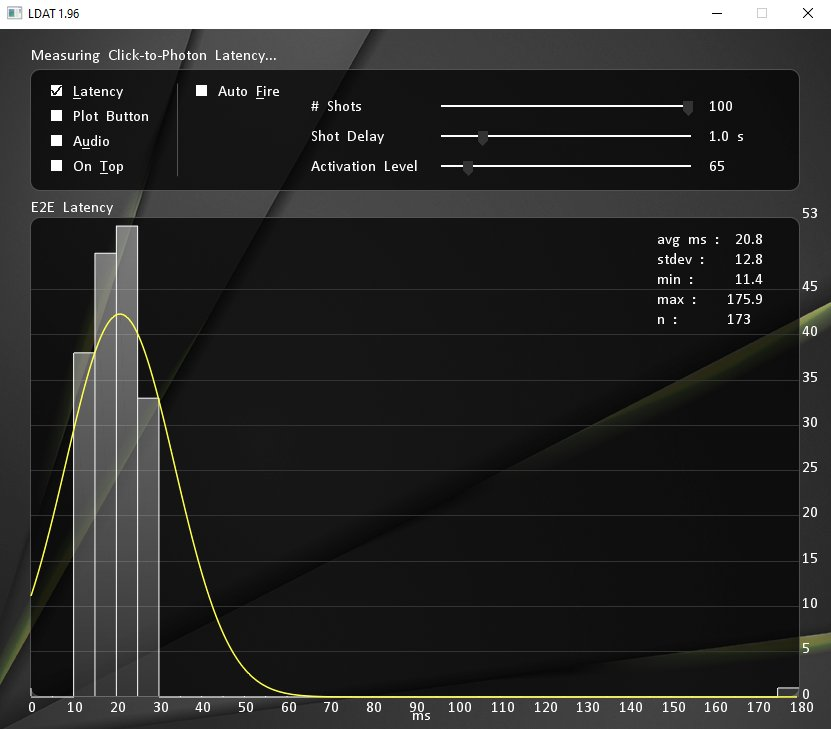
\includegraphics[width=0.8\textwidth]{StatoDellArte_files/nvldat_software.jpg}
	\caption{Screenshot del software Nvidia LDAT (da igorslab.de)}
	\label{fig:nvldat_software}
\end{figure}

Il dispositivo è stato aggiornato intorno a Maggio 2021, con un case di plastica non stampata e l'aggiunta di un pulsante sulla parte frontale del dispositivo per interagire con il software Nvidia LDAT mentre il dispositivo esegue i test e la possibilità di collegare un sensore di luminosità esterno. Per il resto, il dispositivo sembra invariato. La figura \ref{fig:nvldat_v2} mostra il nuovo case.

\begin{figure}[h!]
	\centering
	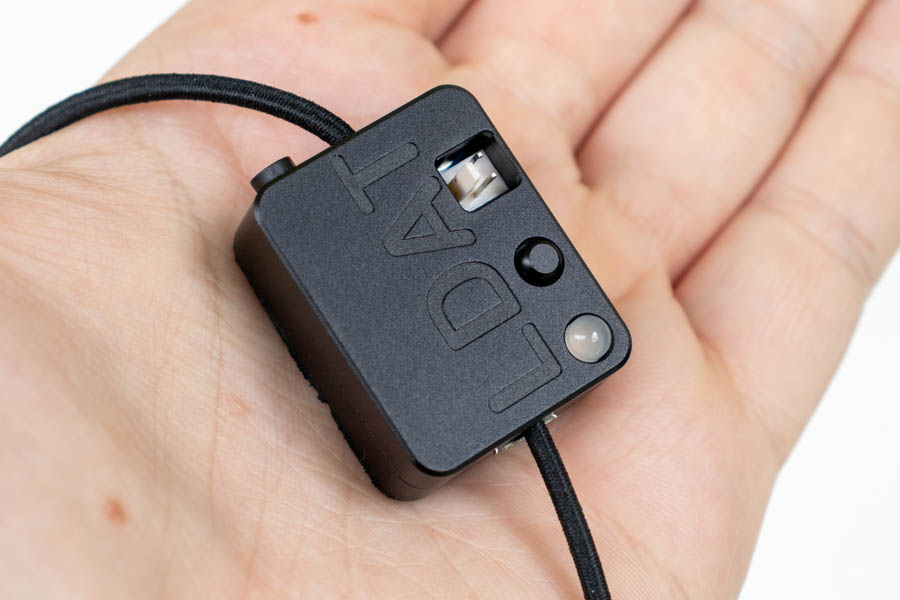
\includegraphics[width=0.8\textwidth]{StatoDellArte_files/nvldat_v2.jpg}
	\caption{Nuova versione di Nvidia LDAT (da techpowerup.com)}
	\label{fig:nvldat_v2}
\end{figure}

Nvidia purtroppo ha scelto di non commercializzare nessuna versione di questo dispositivo, ma lo ha solo distribuito ad alcuni giornalisti di tecnologia come parte di un \textit{``reviewers kit''}, ma ha creato Nvidia Reflex Latency Analyzer, una sorta di versione \textit{built-in} in alcuni monitor e mouse compatibili che è in grado di misurare la latenza senza bisogno di dispositivi esterni.

Nvidia Reflex Latency Analyzer\footnote{\url{https://www.nvidia.com/en-us/geforce/news/reflex-latency-analyzer-360hz-g-sync-monitors/}} consente ai display con certificazione G-Sync Ultimate (ossia con un processore Nvidia dedicato al loro interno) di eseguire il lavoro che normalmente svolgerebbe il sensore di luminosità, monitorando una piccola area dell'immagine per rilevare variazioni di luminosità. Un mouse compatibile deve essere collegato al display stesso, e il software sarà in grado di misurare il ritardo dell'intero sistema.\\
Il requisito di un mouse esplicitamente supportato da Nvidia è necessaria al software per poter conoscere quanto del ritardo è causato dal mouse stesso e quanto dal resto del sistema. Il tempo di latenza calcolato da questo sistema è sostanzialmente lo stesso che verrebbe misurato con un dispositivo esterno come Nvidia LDAT, a meno di pochi millisecondi dovuti al tempo di risposta dei pixel del display. La figura \ref{fig:nvreflex_example} mostra un overlay con la latenza posizionato da Nvidia Geforce Experience sopra un'applicazione.

\begin{figure}[h!]
	\centering
	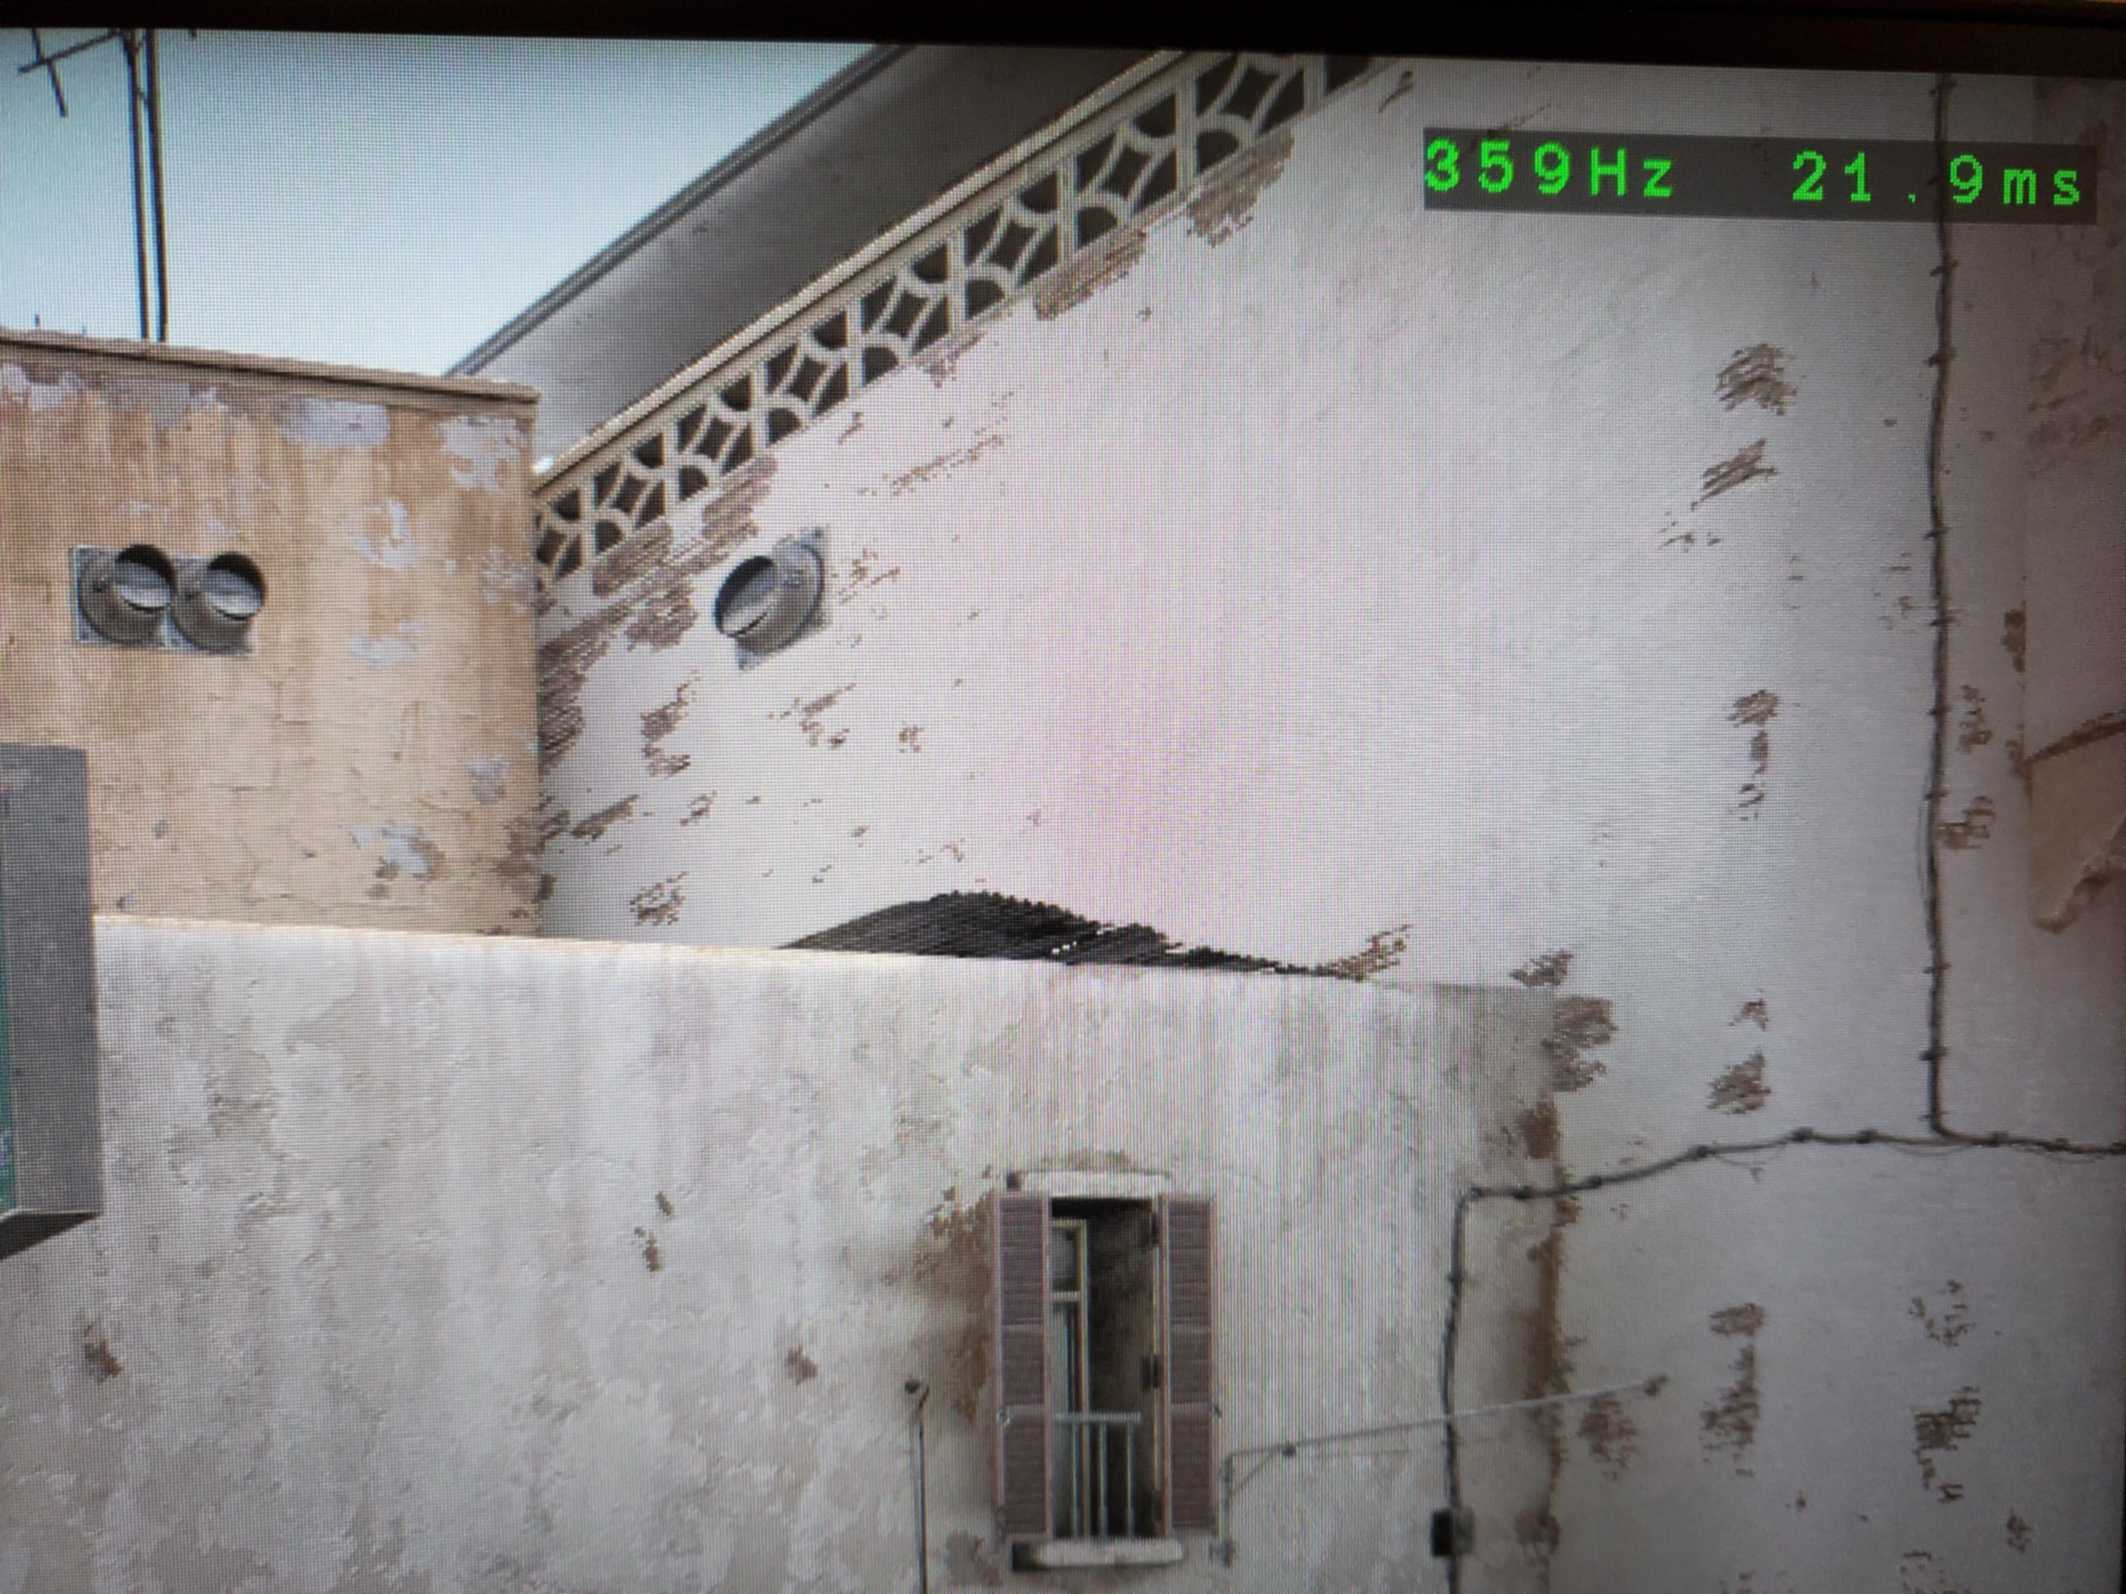
\includegraphics[width=0.8\textwidth]{StatoDellArte_files/nvreflex_example.jpg}
	\caption{Nvidia Reflex Latency Analyzer (da nvidia.com)}
	\label{fig:nvreflex_example}
\end{figure}

Nel momento in cui viene scritto questo paragrafo (aggiornato a Giugno 2021), Nvidia Reflex Latency Analyzer è sostanzialmente inesistente sul mercato poiché supporta pochi modelli di display e mouse, e sono molto costosi per quello che offrono. Il requisito di utilizzare Nvidia Geforce Experience per utilizzarlo, un'applicazione proprietaria che richiede un login e con una pessima reputazione, non ha sicuramente contribuito alla sua diffusione.

\section{DisplayCAL}
DisplayCAL\footnote{\url{https://displaycal.net/}} è un software libero di calibrazione e profilazione di display basato su ArgyllCMS\footnote{\url{https://www.argyllcms.com/}}.

Lo scopo principale di questa applicazione è quella di misurare l'accuratezza dei colori del display utilizzando un colorimetro o uno spettrofotometro tra quelli supportati da ArgyllCMS e generare un profilo di colore ICC che può essere utilizzato nel sistema operativo per fornire dei colori più accurati. Oltre alla calibrazione, può generare anche dei \textit{report} che mostrano il gamut del display, le curve di gamma, e molto altro, secondo molti standard.

La figura \ref{fig:displaycal_report_example} mostra un esempio di \textit{report} generato da DisplayCAL riguardante l'accuratezza dei colori. Il test consiste nel visualizzare una serie di colori e calcolare la differenza tra il colore visualizzato e quello inteso utilizzando qualche tecnica come Delta-E 1976, tenendo conto dello spazio colore in cui deve essere visualizzato.

\begin{figure}[h!]
	\centering
	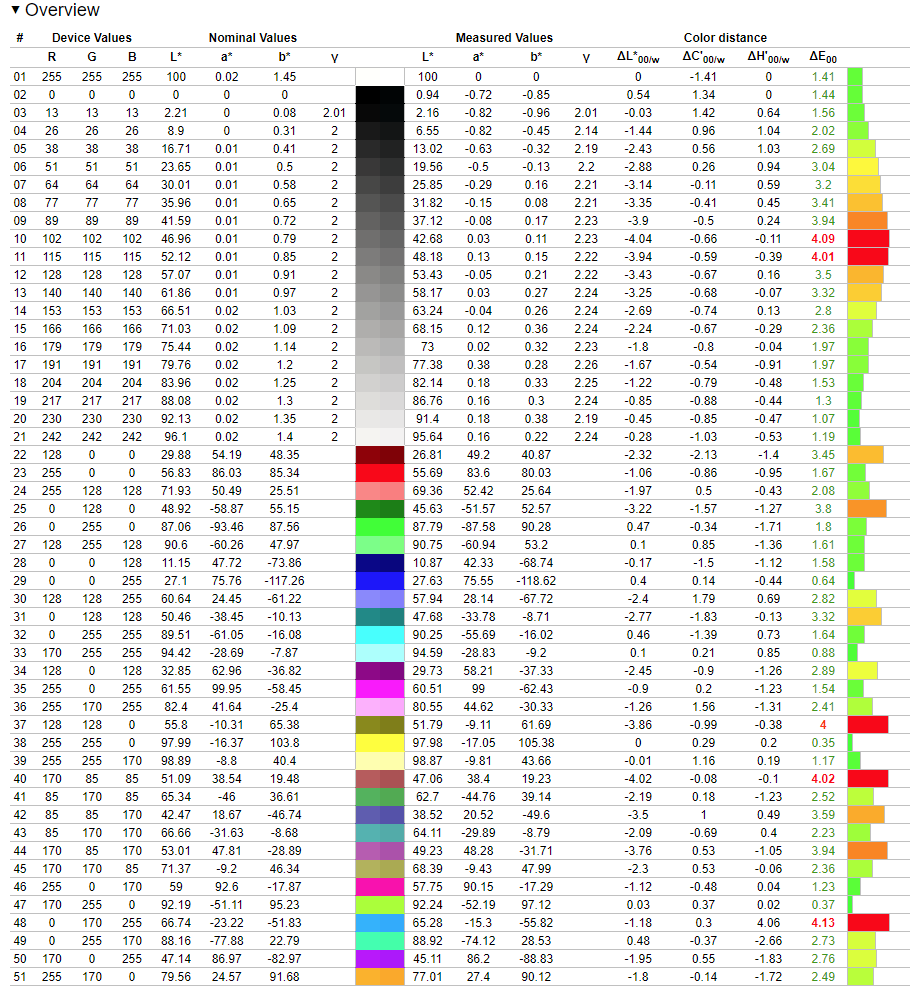
\includegraphics[width=0.8\textwidth]{StatoDellArte_files/displaycal_report_example.png}
	\caption{Esempio di \textit{report} sull'accuratezza dei colori di DisplayCAL}
	\label{fig:displaycal_report_example}
\end{figure}

Siccome questo software si concentra sulla qualità dell'immagine e soprattutto dei colori, il suo obiettivo è diverso rispetto a quello di Nvidia LDAT e di OpenLDAT, e non implementa alcun test riguardante le tempistiche del display e del sistema (Marzo 2021). I dispositivi supportati da DisplayCAL inoltre sono molto più sofisticati e piuttosto costosi, con i modelli più economici (dei colorimetri a tre canali) che partono da circa 100€.

\section{Dispositivo di RTINGS}
Il sito di recensioni RTINGS\footnote{\url{https://rtings.com/}} ha sviluppato un proprio dispositivo per eseguire diversi tipi di misurazioni sui display: tempi di latenza, tempi di risposta dei pixel, errore di transizione causato dall'\textit{overdrive}, e altro.

Purtroppo non sono note informazioni sul dispositivo stesso, ma è visibile in alcune fotografie presenti nelle recensioni, come quella in figura \ref{fig:rtings_device}. Sembra essere un sistema composto da un'MCU e da un sensore di luminosità. Non è noto come i dati raccolti dal sensore vengano analizzati (manualmente o da un programma apposito).

\begin{figure}[h!]
	\centering
	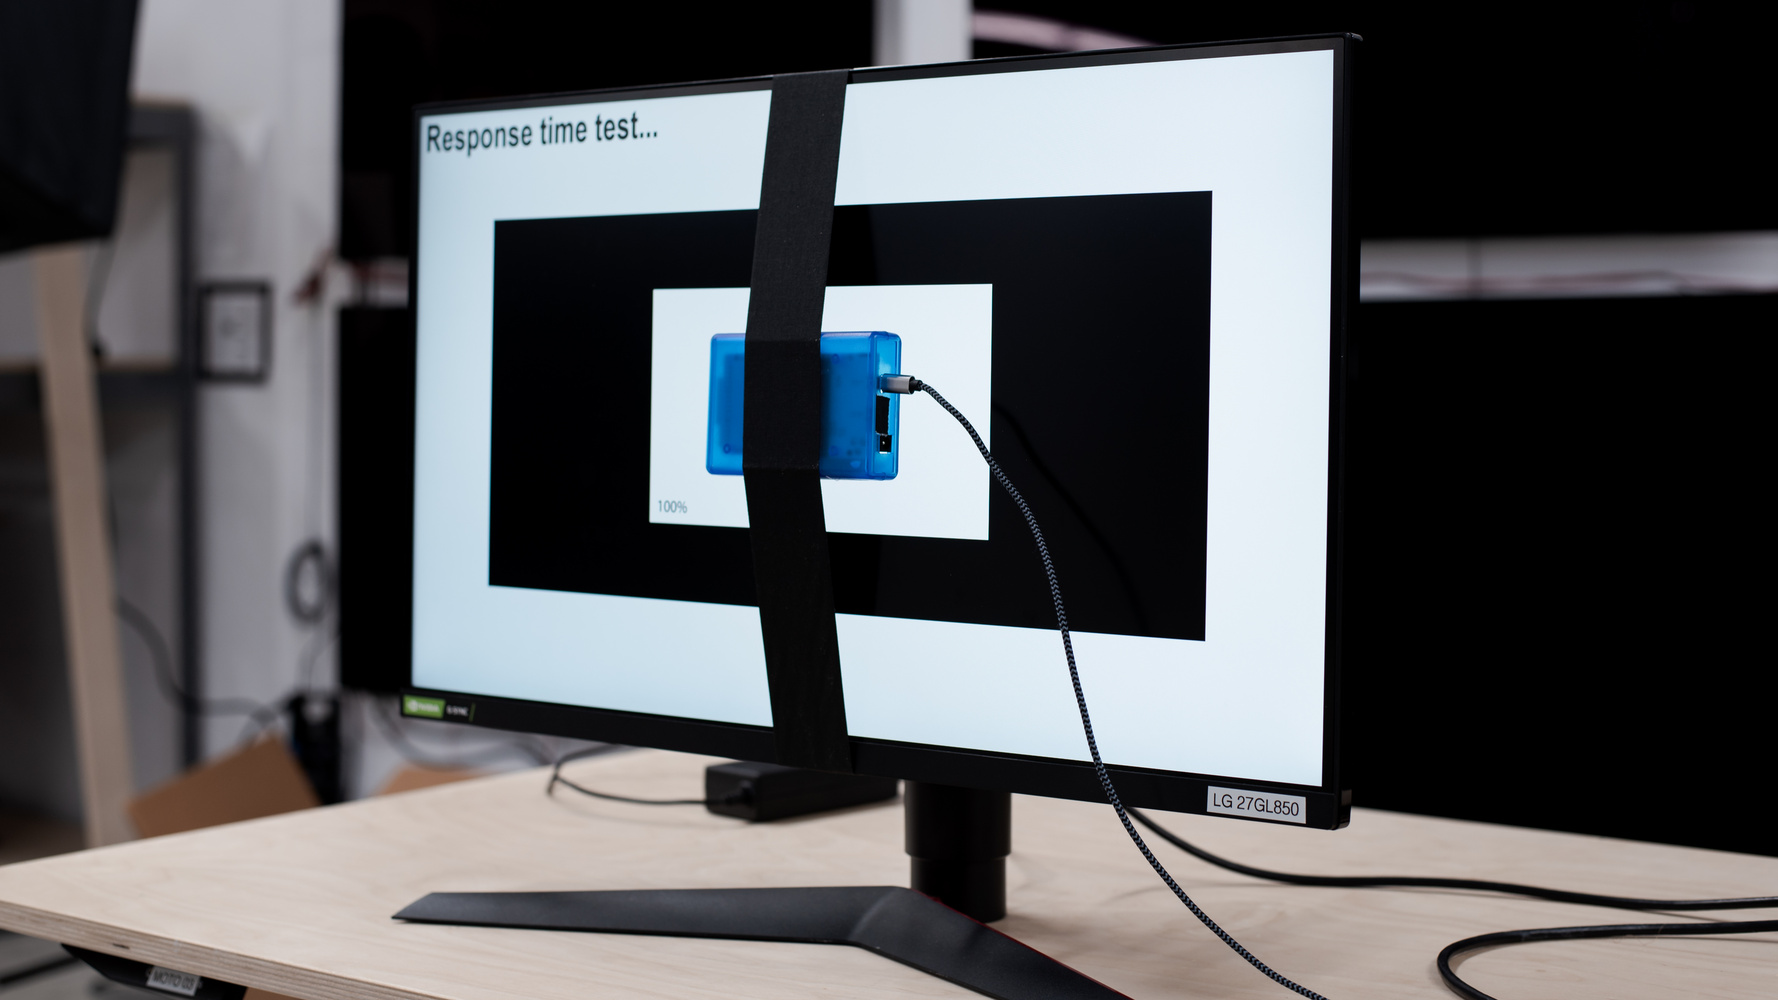
\includegraphics[width=0.8\textwidth]{StatoDellArte_files/rtings_device.jpg}
	\caption{Il dispositivo di RTINGS}
	\label{fig:rtings_device}
\end{figure}

Altri test nelle recensioni presenti sul sito vengono invece svolti utilizzando un colorimetro e DisplayCAL: luminosità, contrasto, curve di gamma, gamut, temperatura del bianco, e altro. Alcuni test infine sono eseguiti manualmente con una telecamera, come quello sugli angoli di visione.

Questo conclude il capitolo sullo stato dell'arte. I capitoli successivi si concentrano sul progetto OpenLDAT.
